\documentclass{beamer}

%
% Common preamble for all three parts.
%


\usepackage{amsmath}
\usepackage{color}
\usepackage{minted}
\usepackage{hyperref}
\usepackage{multicol}
\usepackage{tabularx}
\usepackage{tikz}
\usepackage[utf8]{inputenc}
\usepackage[greek,english]{babel}

\newcommand{\en}{\selectlanguage{english}}
\newcommand{\gr}{\selectlanguage{greek}}

% only inline todonotes work
\usepackage{xkeyval}
\usepackage[textsize=small]{todonotes}
\presetkeys{todonotes}{inline}{}

\usetikzlibrary{shapes,arrows,positioning,shadows}

% no nav buttons
\usenavigationsymbolstemplate{}

\newcommand{\bftt}[1]{\textbf{\texttt{#1}}}
\newcommand{\comment}[1]{{\color[HTML]{008080}\textit{\textbf{\texttt{#1}}}}}
\newcommand{\cmd}[1]{{\color[HTML]{008000}\bftt{#1}}}
\newcommand{\bs}{\char`\\}
\newcommand{\cmdbs}[1]{\cmd{\bs#1}}
\newcommand{\lcb}{\char '173}
\newcommand{\rcb}{\char '175}
\newcommand{\cmdbegin}[1]{\cmdbs{begin\lcb}\bftt{#1}\cmd{\rcb}}
\newcommand{\cmdend}[1]{\cmdbs{end\lcb}\bftt{#1}\cmd{\rcb}}

\newcommand{\wllogo}{\textbf{Overleaf}}

% this is where the example source files are loaded from
% do not include a trailing slash
\newcommand{\fileuri}{https://raw.github.com/jdleesmiller/latex-course/master/en}

\newcommand{\wlserver}{https://www.overleaf.com}
\newcommand{\wlnewdoc}[1]{\wlserver/docs?snip\_uri=\fileuri/#1\&splash=none}

\def\tikzname{Ti\emph{k}Z}

% from http://tex.stackexchange.com/questions/5226/keyboard-font-for-latex
\newcommand*\keystroke[1]{%
  \tikz[baseline=(key.base)]
    \node[%
      draw,
      fill=white,
      drop shadow={shadow xshift=0.25ex,shadow yshift=-0.25ex,fill=black,opacity=0.75},
      rectangle,
      rounded corners=2pt,
      inner sep=1pt,
      line width=0.5pt,
      font=\scriptsize\sffamily
    ](key) {#1\strut}
  ;
}
\newcommand{\keystrokebftt}[1]{\keystroke{\bftt{#1}}}

% stolen from minted.dtx
\newenvironment{exampletwoup}
  {\VerbatimEnvironment
   \begin{VerbatimOut}{example.out}}
  {\end{VerbatimOut}
   \setlength{\parindent}{0pt}
   \fbox{\begin{tabular}{l|l}
   \begin{minipage}{0.55\linewidth}
     \inputminted[fontsize=\small,resetmargins]{latex}{example.out}
   \end{minipage} &
   \begin{minipage}{0.35\linewidth}
     \input{example.out}
   \end{minipage}
   \end{tabular}}}

\newenvironment{exampletwouptiny}
  {\VerbatimEnvironment
   \begin{VerbatimOut}{example.out}}
  {\end{VerbatimOut}
   \setlength{\parindent}{0pt}
   \fbox{\begin{tabular}{l|l}
   \begin{minipage}{0.55\linewidth}
     \inputminted[fontsize=\scriptsize,resetmargins]{latex}{example.out}
   \end{minipage} &
   \begin{minipage}{0.35\linewidth}
     \setlength{\parskip}{6pt plus 1pt minus 1pt}%
     \raggedright\scriptsize\input{example.out}
   \end{minipage}
   \end{tabular}}}

\newenvironment{exampletwouptinynoframe}
  {\VerbatimEnvironment
   \begin{VerbatimOut}{example.out}}
  {\end{VerbatimOut}
   \setlength{\parindent}{0pt}
   \begin{tabular}{l|l}
   \begin{minipage}{0.55\linewidth}
     \inputminted[fontsize=\scriptsize,resetmargins]{latex}{example.out}
   \end{minipage} &
   \begin{minipage}{0.35\linewidth}
     \setlength{\parskip}{6pt plus 1pt minus 1pt}%
     \raggedright\scriptsize\input{example.out}
   \end{minipage}
   \end{tabular}}

\title{ Μια διαδραστική εισαγωγή στο \LaTeX}

\author{\textlatin{Dr John D. Lees-Miller} \\ 
\small {Μετάφραση : Αθανάσιος Παρασκευόπουλος \\(μεταπτυχιακός φοιτητής του ΕΑΠ)}}

\titlegraphic{%

\includegraphics[height=36pt]{overleaf}\\[1em]

\includegraphics[height=24pt]{UoB-logo}
}



\subtitle{Μέρος 2: Δομή Εγγράφων \& Άλλα}

\begin{document}
\gr
%%%%%%%%%%%%%%%%%%%%%%%%%%%%%%%%%%%%%%%%%%%%%%%%%%%%%%%%%%%%%%%%%%%%%%%%%%%%%%%
%%%%%%%%%%%%%%%%%%%%%%%%%%%%%%%%%%%%%%%%%%%%%%%%%%%%%%%%%%%%%%%%%%%%%%%%%%%%%%%
%%%%%%%%%%%%%%%%%%%%%%%%%%%%%%%%%%%%%%%%%%%%%%%%%%%%%%%%%%%%%%%%%%%%%%%%%%%%%%%
\begin{frame}
\titlepage
\end{frame}
\gr
%%%%%%%%%%%%%%%%%%%%%%%%%%%%%%%%%%%%%%%%%%%%%%%%%%%%%%%%%%%%%%%%%%%%%%%%%%%%%%%
%%%%%%%%%%%%%%%%%%%%%%%%%%%%%%%%%%%%%%%%%%%%%%%%%%%%%%%%%%%%%%%%%%%%%%%%%%%%%%%
%%%%%%%%%%%%%%%%%%%%%%%%%%%%%%%%%%%%%%%%%%%%%%%%%%%%%%%%%%%%%%%%%%%%%%%%%%%%%%%
\section{Δομή Εγγράφων}

%%%%%%%%%%%%%%%%%%%%%%%%%%%%%%%%%%%%%%%%%%%%%%%%%%%%%%%%%%%%%%%%%%%%%%%%%%%%%%%
%%%%%%%%%%%%%%%%%%%%%%%%%%%%%%%%%%%%%%%%%%%%%%%%%%%%%%%%%%%%%%%%%%%%%%%%%%%%%%%
%%%%%%%%%%%%%%%%%%%%%%%%%%%%%%%%%%%%%%%%%%%%%%%%%%%%%%%%%%%%%%%%%%%%%%%%%%%%%%%
\begin{frame}{Περιγραφή}
\begin{multicols}{2}
\tableofcontents[currentsection]
\end{multicols}
\end{frame}

%%%%%%%%%%%%%%%%%%%%%%%%%%%%%%%%%%%%%%%%%%%%%%%%%%%%%%%%%%%%%%%%%%%%%%%%%%%%%%%
%%%%%%%%%%%%%%%%%%%%%%%%%%%%%%%%%%%%%%%%%%%%%%%%%%%%%%%%%%%%%%%%%%%%%%%%%%%%%%%
%%%%%%%%%%%%%%%%%%%%%%%%%%%%%%%%%%%%%%%%%%%%%%%%%%%%%%%%%%%%%%%%%%%%%%%%%%%%%%%
\begin{frame}{\insertsection}
\begin{itemize}
\item Στο Μέρος 1, μάθαμε για εντολές και περιβάλλοντα για τη στοιχειοθεσία κειμένου
και τα μαθηματικά.
\item Τώρα, θα μάθουμε για εντολές και περιβάλλοντα για τη δομή των εγγράφων.
\item Μπορείτε να δοκιμάσετε τις νέες εντολές στο \en Overleaf \gr:
\end{itemize}
\vskip 2em
\begin{center}
\fbox{\href{\wlnewdoc{basics.tex}}{%
Κάντε κλικ εδώ για να ανοίξετε το παράδειγμα \en \wllogo{}}}\gr
\\[1ex]\scriptsize{}
Για καλύτερα αποτελέσματα, χρησιμοποιήστε \en \href{http://www.google.com/chrome}{Google Chrome} \gr  ή \en \href{http://www.mozilla.org/en-US/firefox/new/}{FireFox}.\gr
\end{center}
\vskip 2ex
\begin{itemize}
\item Ας αρχίσουμε!
\end{itemize}
\end{frame}

%%%%%%%%%%%%%%%%%%%%%%%%%%%%%%%%%%%%%%%%%%%%%%%%%%%%%%%%%%%%%%%%%%%%%%%%%%%%%%%
%%%%%%%%%%%%%%%%%%%%%%%%%%%%%%%%%%%%%%%%%%%%%%%%%%%%%%%%%%%%%%%%%%%%%%%%%%%%%%%
%%%%%%%%%%%%%%%%%%%%%%%%%%%%%%%%%%%%%%%%%%%%%%%%%%%%%%%%%%%%%%%%%%%%%%%%%%%%%%%
\subsection{Τίτλος και Περίληψη}
\begin{frame}[fragile]{\insertsubsection}
\begin{itemize}{\small
\item Δώστε στο \LaTeX{} τα ονόματα του \en \cmdbs{title} \gr και \en \cmdbs{author}\gr στο προοίμιο.
\item Στη συνέχεια χρησιμοποιήστε το \cmdbs\en {maketitle}\gr στο έγγραφο για να δημιουργήσετε πραγματικά τον τίτλο.
\item Χρησιμοποιήστε το περιβάλλον \en \bftt{abstract}\gr για να κάνετε μια περίληψη.
}\end{itemize}
\en
\begin{minipage}{0.55\linewidth}
\inputminted[fontsize=\scriptsize,frame=single,resetmargins]{latex}%
  {structure-title.tex}
\end{minipage}
\begin{minipage}{0.35\linewidth}

\includegraphics[width=\textwidth,clip,trim=2.2in 7in 2.2in 2in]{structure-title.pdf}
\end{minipage}
\end{frame}
\gr
%%%%%%%%%%%%%%%%%%%%%%%%%%%%%%%%%%%%%%%%%%%%%%%%%%%%%%%%%%%%%%%%%%%%%%%%%%%%%%%
%%%%%%%%%%%%%%%%%%%%%%%%%%%%%%%%%%%%%%%%%%%%%%%%%%%%%%%%%%%%%%%%%%%%%%%%%%%%%%%
%%%%%%%%%%%%%%%%%%%%%%%%%%%%%%%%%%%%%%%%%%%%%%%%%%%%%%%%%%%%%%%%%%%%%%%%%%%%%%%
\subsection{Ενότητες}
\begin{frame}{\insertsubsection}
\begin{itemize}{\small
\item Απλώς χρησιμοποιήστε τις \en \cmdbs{section} \gr και \en \cmdbs{subsection}\gr.
\item Μπορείτε να μαντέψετε τι κάνουν οι \en \cmdbs{section*}\gr και \en \cmdbs{subsection*}\gr$;$
}\end{itemize}
\en
\begin{minipage}{0.55\linewidth}
\inputminted[fontsize=\scriptsize,frame=single,resetmargins]{latex}%
  {structure-sections.tex}
\end{minipage}
\begin{minipage}{0.35\linewidth}
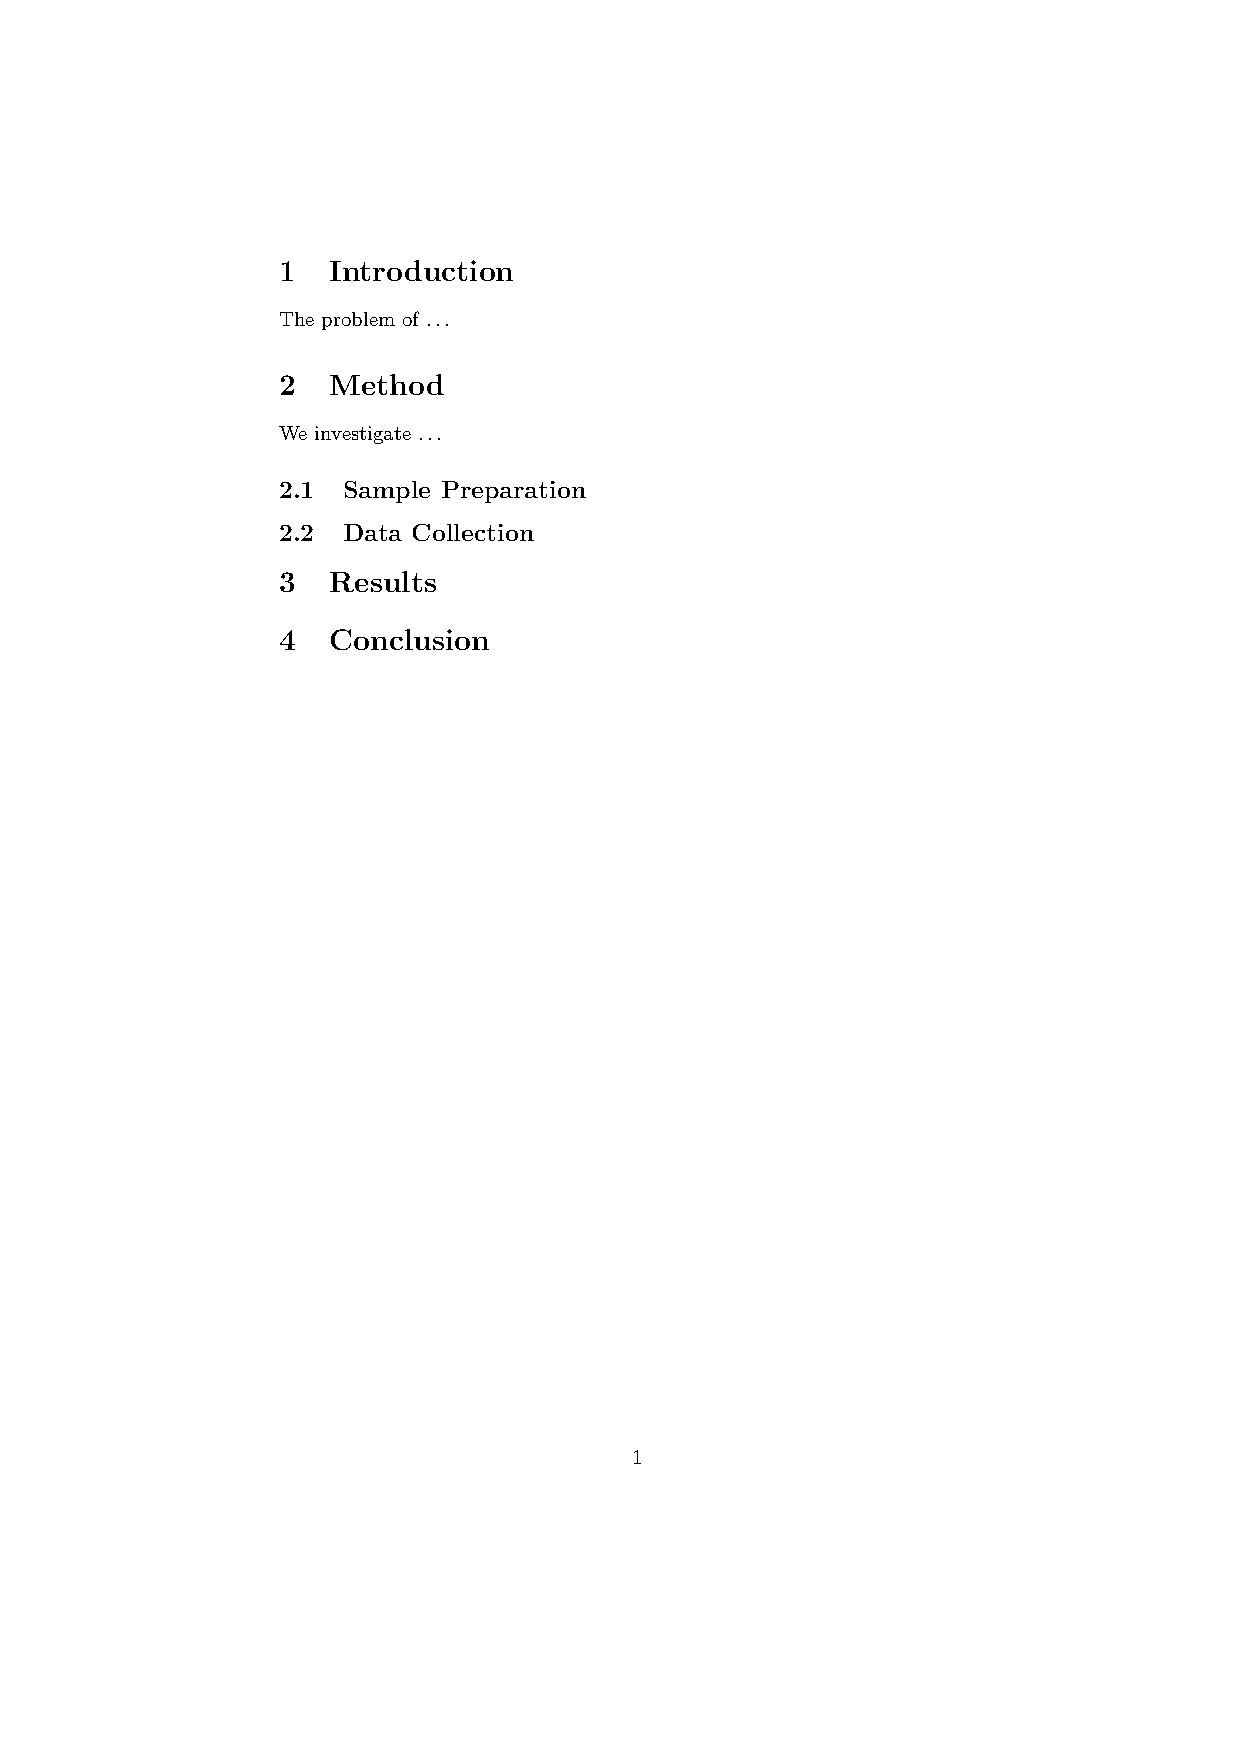
\includegraphics[width=\textwidth,clip,trim=1.5in 6in 4in 1in]{structure-sections.pdf}
\end{minipage}
\end{frame}
\gr
%%%%%%%%%%%%%%%%%%%%%%%%%%%%%%%%%%%%%%%%%%%%%%%%%%%%%%%%%%%%%%%%%%%%%%%%%%%%%%%
%%%%%%%%%%%%%%%%%%%%%%%%%%%%%%%%%%%%%%%%%%%%%%%%%%%%%%%%%%%%%%%%%%%%%%%%%%%%%%%
%%%%%%%%%%%%%%%%%%%%%%%%%%%%%%%%%%%%%%%%%%%%%%%%%%%%%%%%%%%%%%%%%%%%%%%%%%%%%%%
\subsection{Ετικέτες και παραπομπές}
\begin{frame}[fragile]{\insertsubsection}
\begin{itemize}{\small
\item Χρησιμοποιήστε τις \en \cmdbs{label}\gr και \en \cmdbs{ref}\gr \spaceγια αυτόματη αρίθμηση.
\item Το πακέτο \en \bftt{amsmath} \gr \spaceπαρέχει την \en \cmdbs{eqref} \gr για αναφορά εξισώσεων.
}\end{itemize}
\en
\begin{minipage}{0.55\linewidth}
\inputminted[fontsize=\scriptsize,frame=single,resetmargins]{latex}%
  {structure-crossref.tex}
\end{minipage}
\begin{minipage}{0.35\linewidth}
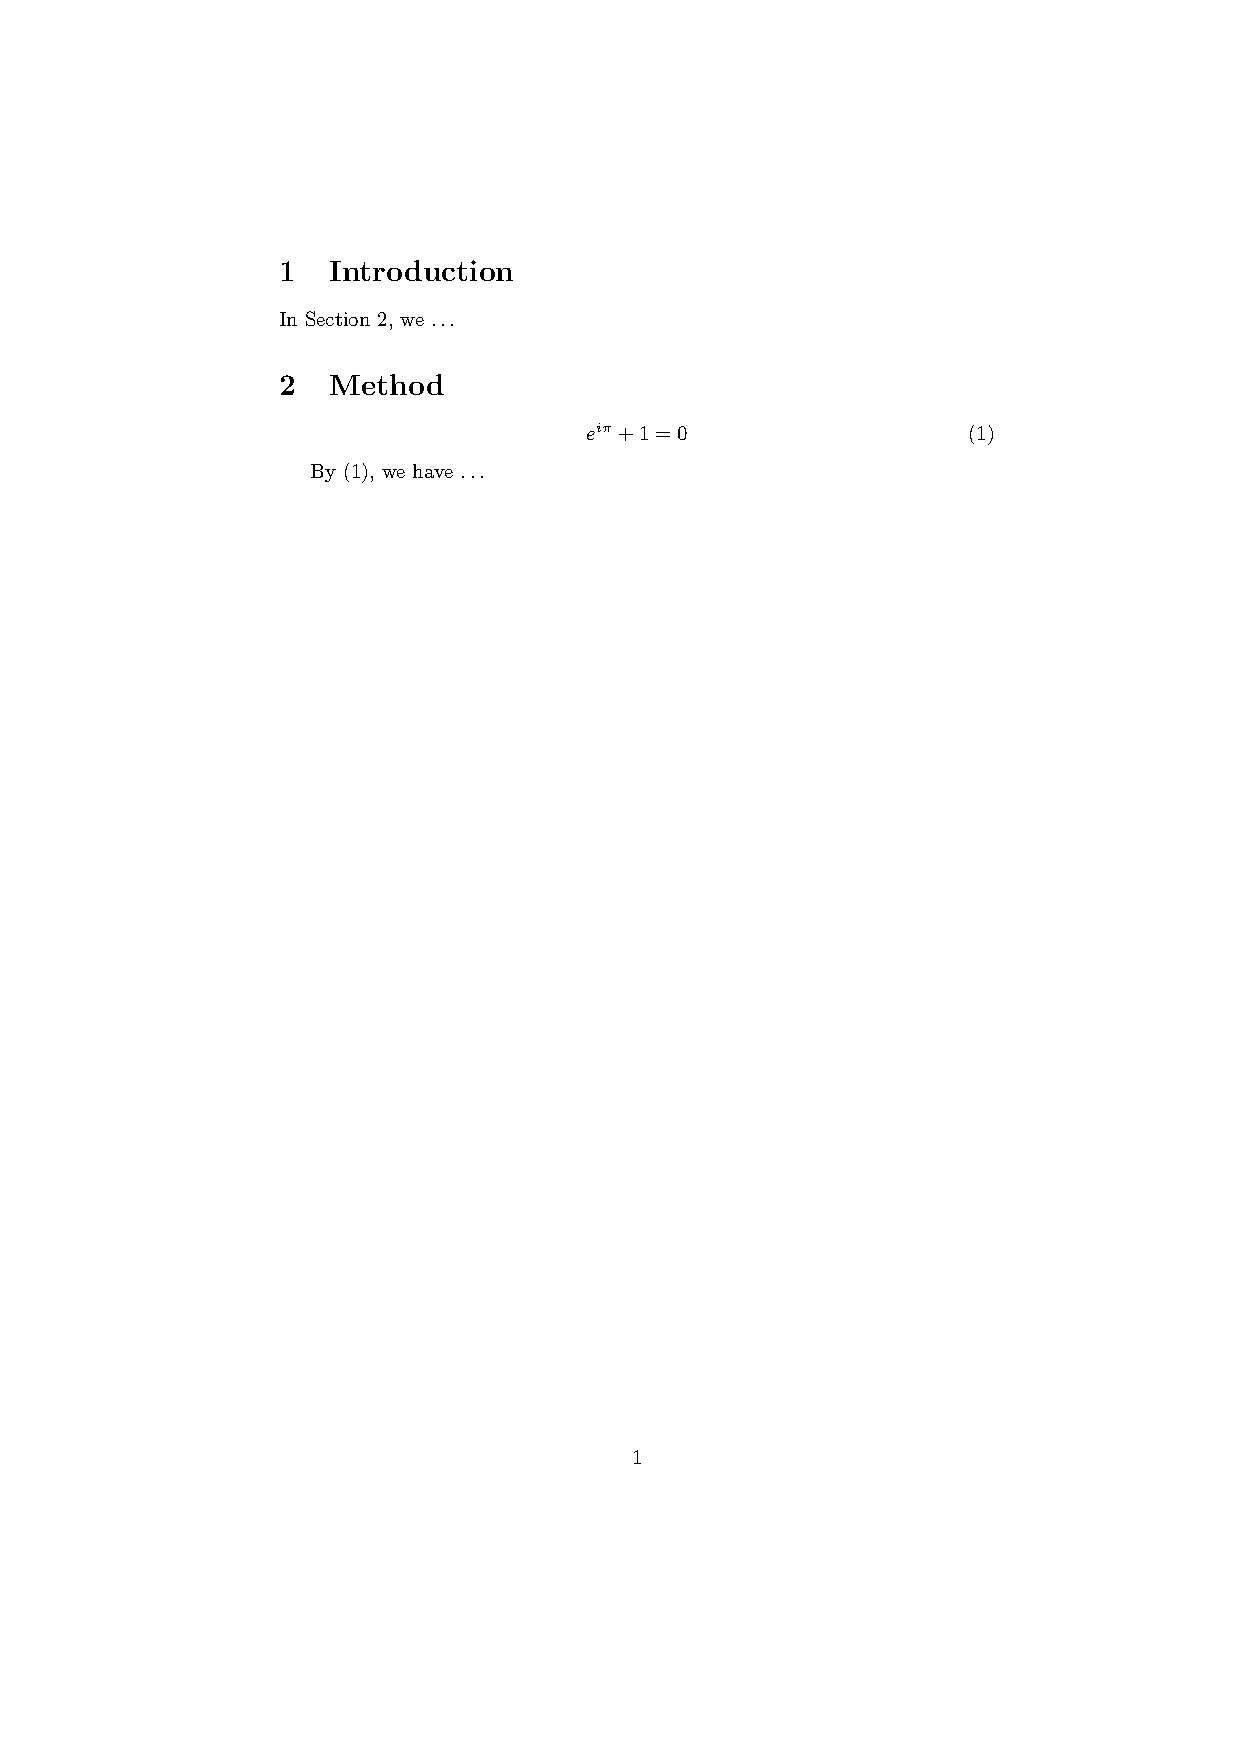
\includegraphics[width=\textwidth,clip,trim=1.8in 6in 1.6in 1in]{structure-crossref.pdf}
\end{minipage}
\end{frame}
\gr
%%%%%%%%%%%%%%%%%%%%%%%%%%%%%%%%%%%%%%%%%%%%%%%%%%%%%%%%%%%%%%%%%%%%%%%%%%%%%%%
%%%%%%%%%%%%%%%%%%%%%%%%%%%%%%%%%%%%%%%%%%%%%%%%%%%%%%%%%%%%%%%%%%%%%%%%%%%%%%%
%%%%%%%%%%%%%%%%%%%%%%%%%%%%%%%%%%%%%%%%%%%%%%%%%%%%%%%%%%%%%%%%%%%%%%%%%%%%%%%
\subsection{'Ασκηση}
\begin{frame}[fragile]{Άσκηση στην Δομή Εγγράφων}

\begin{block}{Πληκτρολογήστε αυτή τη σύντομη εργασία στο \LaTeX:
\en
\footnote{From \url{http://pdos.csail.mit.edu/scigen/}, a random
paper generator.}}\gr
\begin{center}
\fbox{\href{\fileuri/structure-exercise-solution.pdf}{%
Κάντε κλικ για να ανοίξετε την εργασία}}
\end{center}
Κάντε την εργασία σας να μοιάζει με αυτή. Χρησιμοποιήστε τα \en \cmdbs{ref} \gr και \en \cmdbs{eqref} \gr για να αποφύγετε τη ρητή εγγραφή αριθμών ενοτήτων και εξισώσεων στο κείμενο.
\end{block}
\vskip 2ex
\begin{center}
\fbox{\href{\wlnewdoc{structure-exercise.tex}}{%
Κάντε κλικ για να ανοίξετε αυτήν την άσκηση \en\wllogo{}}}\gr
\end{center}

\begin{itemize}
\item Μόλις προσπαθήσετε,
\fbox{\href{\wlnewdoc{structure-exercise-solution.tex}}{%
κάντε κλικ εδώ για να δείτε τη λύση μου}}.
\end{itemize}
\end{frame}

%%%%%%%%%%%%%%%%%%%%%%%%%%%%%%%%%%%%%%%%%%%%%%%%%%%%%%%%%%%%%%%%%%%%%%%%%%%%%%%
%%%%%%%%%%%%%%%%%%%%%%%%%%%%%%%%%%%%%%%%%%%%%%%%%%%%%%%%%%%%%%%%%%%%%%%%%%%%%%%
%%%%%%%%%%%%%%%%%%%%%%%%%%%%%%%%%%%%%%%%%%%%%%%%%%%%%%%%%%%%%%%%%%%%%%%%%%%%%%%
\section{Εικόνες και Πίνακες}

%%%%%%%%%%%%%%%%%%%%%%%%%%%%%%%%%%%%%%%%%%%%%%%%%%%%%%%%%%%%%%%%%%%%%%%%%%%%%%%
%%%%%%%%%%%%%%%%%%%%%%%%%%%%%%%%%%%%%%%%%%%%%%%%%%%%%%%%%%%%%%%%%%%%%%%%%%%%%%%
%%%%%%%%%%%%%%%%%%%%%%%%%%%%%%%%%%%%%%%%%%%%%%%%%%%%%%%%%%%%%%%%%%%%%%%%%%%%%%%
\begin{frame}{Περιγραφή}
\begin{multicols}{2}
\tableofcontents[currentsection]
\end{multicols}
\end{frame}

%%%%%%%%%%%%%%%%%%%%%%%%%%%%%%%%%%%%%%%%%%%%%%%%%%%%%%%%%%%%%%%%%%%%%%%%%%%%%%%
%%%%%%%%%%%%%%%%%%%%%%%%%%%%%%%%%%%%%%%%%%%%%%%%%%%%%%%%%%%%%%%%%%%%%%%%%%%%%%%
%%%%%%%%%%%%%%%%%%%%%%%%%%%%%%%%%%%%%%%%%%%%%%%%%%%%%%%%%%%%%%%%%%%%%%%%%%%%%%%
\subsection{Γραφικά}
\begin{frame}[fragile]{\insertsubsection}
\begin{itemize}
\item Απαιτείται το πακέτο \en \bftt{graphicx}\gr, το οποίο παρέχει την εντολή \en \cmdbs{includegraphics}\gr.
\item Οι υποστηριζόμενες μορφές γραφικών περιλαμβάνουν \en JPEG, PNG \gr και \en PDF\gr (συνήθως).
\end{itemize}
\en
\begin{exampletwouptiny}

\includegraphics[
  width=0.5\textwidth]{gerbil}


\includegraphics[
  width=0.3\textwidth,
  angle=270]{gerbil}
\end{exampletwouptiny}

\tiny{Image license: \href{https://pixabay.com/en/animal-apple-attractive-beautiful-1239390/}{CC0}}
\end{frame}
\gr
%%%%%%%%%%%%%%%%%%%%%%%%%%%%%%%%%%%%%%%%%%%%%%%%%%%%%%%%%%%%%%%%%%%%%%%%%%%%%%%
%%%%%%%%%%%%%%%%%%%%%%%%%%%%%%%%%%%%%%%%%%%%%%%%%%%%%%%%%%%%%%%%%%%%%%%%%%%%%%%
%%%%%%%%%%%%%%%%%%%%%%%%%%%%%%%%%%%%%%%%%%%%%%%%%%%%%%%%%%%%%%%%%%%%%%%%%%%%%%%
\begin{frame}[fragile]{Ενδιάμεσο: Προαιρετικά ορίσματα}
\begin{itemize}
\item Χρησιμοποιούμε αγκύλες \en\keystrokebftt{[} \keystrokebftt{]}\gr για προαιρετικά ορίσματα, αντί για αγκύλες \en \keystrokebftt{\{} \keystrokebftt{\}}\gr.
\item Το \en \cmdbs{includegraphics} \gr δέχεται προαιρετικά ορίσματα που σας επιτρέπουν να μετασχηματίσετε το
εικόνα όταν περιλαμβάνεται. Για παράδειγμα, το \en \bftt{width=0.3\cmdbs{textwidth}}\gr \space κάνει την εικόνα να καταλαμβάνει το 30\% του πλάτους του περιβάλλοντος κειμένου \en(\cmdbs{textwidth})\gr.
\item Το \en\cmdbs{documentclass}\gr δέχεται επίσης προαιρετικά ορίσματα. Παράδειγμα:
\en\mint{latex}|\documentclass[12pt,dwocolumn]{article}|
\vskip 3ex \gr
κάνει το κείμενο μεγαλύτερο \en(12 pt)\gr και το τοποθετεί σε δύο στήλες.
\item Που τα μαθαίνεις αυτά; Δείτε τις διαφάνειες στο τέλος αυτής της παρουσίασης για συνδέσμους για περισσότερες πληροφορίες.
\end{itemize}
\end{frame}

%%%%%%%%%%%%%%%%%%%%%%%%%%%%%%%%%%%%%%%%%%%%%%%%%%%%%%%%%%%%%%%%%%%%%%%%%%%%%%%
%%%%%%%%%%%%%%%%%%%%%%%%%%%%%%%%%%%%%%%%%%%%%%%%%%%%%%%%%%%%%%%%%%%%%%%%%%%%%%%
%%%%%%%%%%%%%%%%%%%%%%%%%%%%%%%%%%%%%%%%%%%%%%%%%%%%%%%%%%%%%%%%%%%%%%%%%%%%%%%
\subsection[fragile]{Σχεδία}
\begin{frame}{\insertsubsection}
\begin{itemize}
\item Επιτρέψτε στο \LaTeX{} να αποφασίσει πού θα πάει η φιγούρα (μπορεί να "επιπλέει").
\item Μπορείτε επίσης να δώσετε στο σχήμα μια λεζάντα, με την οποία μπορείτε να αναφέρετε με
\en \cmdbs{ref} \gr.
\end{itemize}
\en
\begin{minipage}{0.55\linewidth}
\inputminted[fontsize=\scriptsize,frame=single,resetmargins]{latex}%
  {media-graphics.tex}
\end{minipage}
\begin{minipage}{0.35\linewidth}
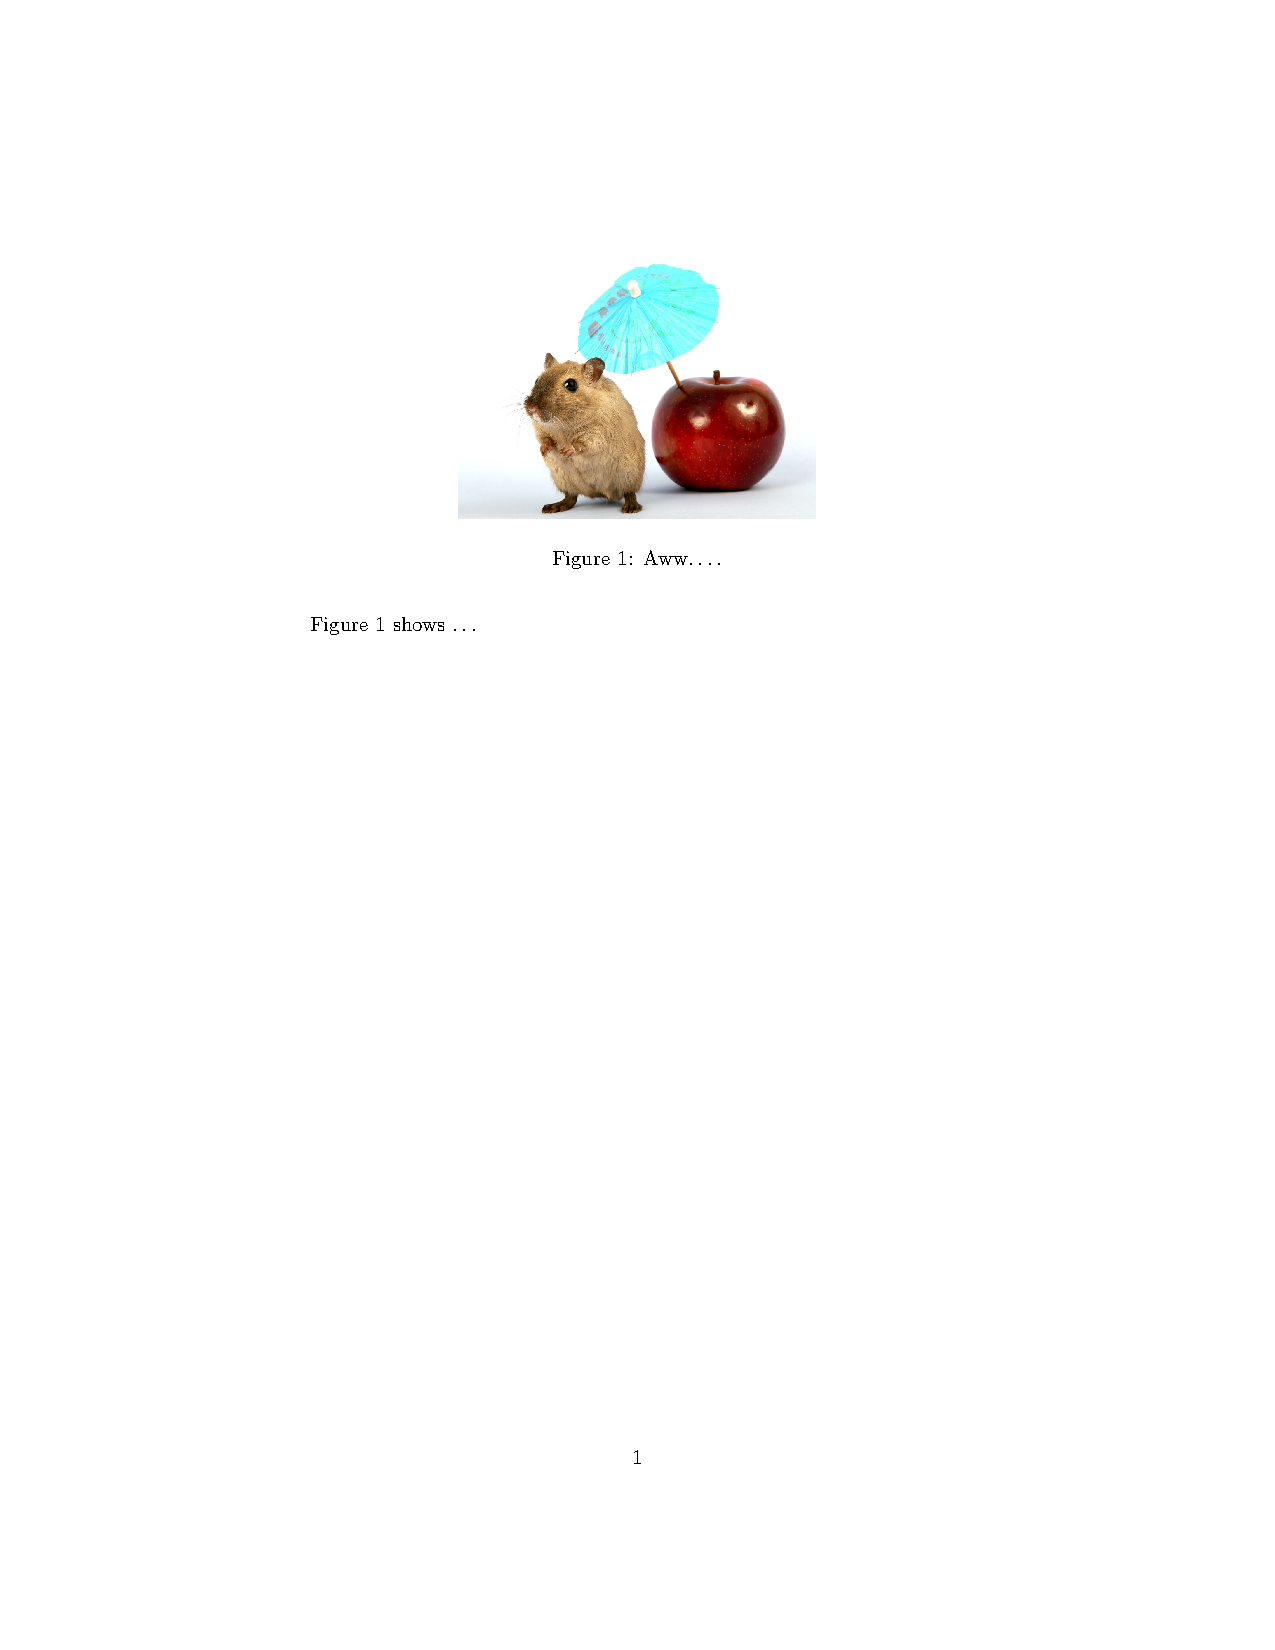
\includegraphics[width=\textwidth,clip,trim=2in 5in 3in 1in]{media-graphics.pdf}
\end{minipage}

\tiny{Image license: \href{https://pixabay.com/en/animal-apple-attractive-beautiful-1239390/}{CC0}}
\end{frame}
\gr
%%%%%%%%%%%%%%%%%%%%%%%%%%%%%%%%%%%%%%%%%%%%%%%%%%%%%%%%%%%%%%%%%%%%%%%%%%%%%%%
%%%%%%%%%%%%%%%%%%%%%%%%%%%%%%%%%%%%%%%%%%%%%%%%%%%%%%%%%%%%%%%%%%%%%%%%%%%%%%%
%%%%%%%%%%%%%%%%%%%%%%%%%%%%%%%%%%%%%%%%%%%%%%%%%%%%%%%%%%%%%%%%%%%%%%%%%%%%%%%
\subsection{Πίνακες}
\begin{frame}[fragile]{\insertsubsection}
\begin{itemize}
\item Οι πίνακες στο \LaTeX{} χρειάζονται λίγη εξοικείωση.
\item Χρησιμοποιήστε το περιβάλλον \en \bftt{tabular}\gr \spaceαπό το πακέτο \en \bftt{tabularx}\gr.
\item 
Το όρισμα καθορίζει τη στοίχιση στηλών --- \en \textbf{l}eft, \textbf{r}right, \textbf{r}right \gr.
\en
\begin{exampletwouptiny}
\begin{tabular}{lrr}
Item   & Qty & Unit \$ \\
Widget & 1   & 199.99  \\
Gadget & 2   & 399.99  \\
Cable  & 3   & 19.99   \\
\end{tabular}
\end{exampletwouptiny}
\gr
\item Χρησιμοποιήστε το\en \cmdbs{hline} \gr για οριζόντιες γραμμές.
\en
\begin{exampletwouptiny}
\begin{tabular}{|l|r|r|} \hline
Item   & Qty & Unit \$ \\\hline
Widget & 1   & 199.99  \\
Gadget & 2   & 399.99  \\
Cable  & 3   & 19.99   \\\hline
\end{tabular}
\end{exampletwouptiny}
\gr
\item Χρησιμοποιήστε ένα συμπλεκτικό σύμβολο \keystrokebftt{\&} για να διαχωρίσετε στήλες και μια διπλή ανάστροφη κάθετο \en \keystrokebftt{\bs}\keystrokebftt{\bs} \gr για να ξεκινήσετε μια νέα σειρά.
\end{itemize}
\end{frame}

%%%%%%%%%%%%%%%%%%%%%%%%%%%%%%%%%%%%%%%%%%%%%%%%%%%%%%%%%%%%%%%%%%%%%%%%%%%%%%%
%%%%%%%%%%%%%%%%%%%%%%%%%%%%%%%%%%%%%%%%%%%%%%%%%%%%%%%%%%%%%%%%%%%%%%%%%%%%%%%
%%%%%%%%%%%%%%%%%%%%%%%%%%%%%%%%%%%%%%%%%%%%%%%%%%%%%%%%%%%%%%%%%%%%%%%%%%%%%%%
\addtocontents{toc}{\newpage}
\section{Βιβλιογραφίες}

%%%%%%%%%%%%%%%%%%%%%%%%%%%%%%%%%%%%%%%%%%%%%%%%%%%%%%%%%%%%%%%%%%%%%%%%%%%%%%%
%%%%%%%%%%%%%%%%%%%%%%%%%%%%%%%%%%%%%%%%%%%%%%%%%%%%%%%%%%%%%%%%%%%%%%%%%%%%%%%
%%%%%%%%%%%%%%%%%%%%%%%%%%%%%%%%%%%%%%%%%%%%%%%%%%%%%%%%%%%%%%%%%%%%%%%%%%%%%%%
\begin{frame}{Περιγραφή}
\begin{multicols}{2}
\tableofcontents[currentsection]
\end{multicols}
\end{frame}

%%%%%%%%%%%%%%%%%%%%%%%%%%%%%%%%%%%%%%%%%%%%%%%%%%%%%%%%%%%%%%%%%%%%%%%%%%%%%%%
%%%%%%%%%%%%%%%%%%%%%%%%%%%%%%%%%%%%%%%%%%%%%%%%%%%%%%%%%%%%%%%%%%%%%%%%%%%%%%%
%%%%%%%%%%%%%%%%%%%%%%%%%%%%%%%%%%%%%%%%%%%%%%%%%%%%%%%%%%%%%%%%%%%%%%%%%%%%%%%
\en
\subsection { bib\TeX} \gr
\begin{frame}[fragile]{\en \insertsubsection{} \gr 1}
\begin{itemize}
\item Τοποθετήστε τις αναφορές σας σε ένα αρχείο \en \bftt{.bib}\gr σε μορφή βάσης δεδομένων \en «bibtex»:
\inputminted[fontsize=\scriptsize,frame=single]{latex}{bib-example.bib}\gr
\item Οι περισσότεροι διαχειριστές αναφοράς μπορούν να εξάγουν σε μορφή \en bibtex \gr.
\end{itemize}
\end{frame}

%%%%%%%%%%%%%%%%%%%%%%%%%%%%%%%%%%%%%%%%%%%%%%%%%%%%%%%%%%%%%%%%%%%%%%%%%%%%%%%
%%%%%%%%%%%%%%%%%%%%%%%%%%%%%%%%%%%%%%%%%%%%%%%%%%%%%%%%%%%%%%%%%%%%%%%%%%%%%%%
%%%%%%%%%%%%%%%%%%%%%%%%%%%%%%%%%%%%%%%%%%%%%%%%%%%%%%%%%%%%%%%%%%%%%%%%%%%%%%%
\begin{frame}[fragile]{\en\insertsubsection{}\gr 2}
\begin{itemize}
\item Κάθε καταχώρηση στο αρχείο \en\bftt{.bib} \gr έχει ένα \en \emph{key} \gr για το οποίο μπορείτε να χρησιμοποιήσετε
αναφερθείτε στο έγγραφο. Για παράδειγμα, το \en \bftt{Jacobson1999Towards}\gr \spaceείναι το κλειδί για αυτό το άρθρο:
\en
\begin{minted}[fontsize=\small,frame=single]{latex}
@Article{Jacobson1999Towards,
  author = {Van Jacobson},
  ...
}
\end{minted}
\gr
\item Είναι καλή ιδέα να χρησιμοποιήσετε ένα κλειδί με βάση το όνομα, το έτος και τον τίτλο.
\item Το \LaTeX{} μπορεί να μορφοποιήσει αυτόματα τις αναφορές εντός κειμένου και να δημιουργήσει ένα
κατάλογος αναφορών, γνωρίζει τα περισσότερα τυπικά στυλ αλλά μπορείτε να σχεδιάσετε και το δικό σας.
\end{itemize}
\end{frame}

%%%%%%%%%%%%%%%%%%%%%%%%%%%%%%%%%%%%%%%%%%%%%%%%%%%%%%%%%%%%%%%%%%%%%%%%%%%%%%%
%%%%%%%%%%%%%%%%%%%%%%%%%%%%%%%%%%%%%%%%%%%%%%%%%%%%%%%%%%%%%%%%%%%%%%%%%%%%%%%
%%%%%%%%%%%%%%%%%%%%%%%%%%%%%%%%%%%%%%%%%%%%%%%%%%%%%%%%%%%%%%%%%%%%%%%%%%%%%%%
\begin{frame}[fragile]{\en \insertsubsection{} \gr 3}
\begin{itemize}
\item Χρησιμοποιήστε το πακέτο \en \bftt{natbib}\gr \footnote{Υπάρχει ένα νέο πακέτο με περισσότερες δυνατότητες το \en \bftt{biblatex} \gr αλλά τα περισσότερα από τα πρότυπα άρθρων να χρησιμοποιούν
   \en \bftt{natbib}.\gr} με \en \cmdbs{citet}\gr και \en \cmdbs{citep}.\gr
\item Ανατρέξτε στο \en \cmdbs{bibliography}\gr \space στο τέλος και καθορίστε ένα \en \cmdbs{bibliographystyle}\gr.
\end{itemize}
\en
\begin{minipage}{0.55\linewidth}
\inputminted[fontsize=\scriptsize,frame=single,resetmargins]{latex}%
  {bib-example.tex}
\end{minipage}
\begin{minipage}{0.35\linewidth}
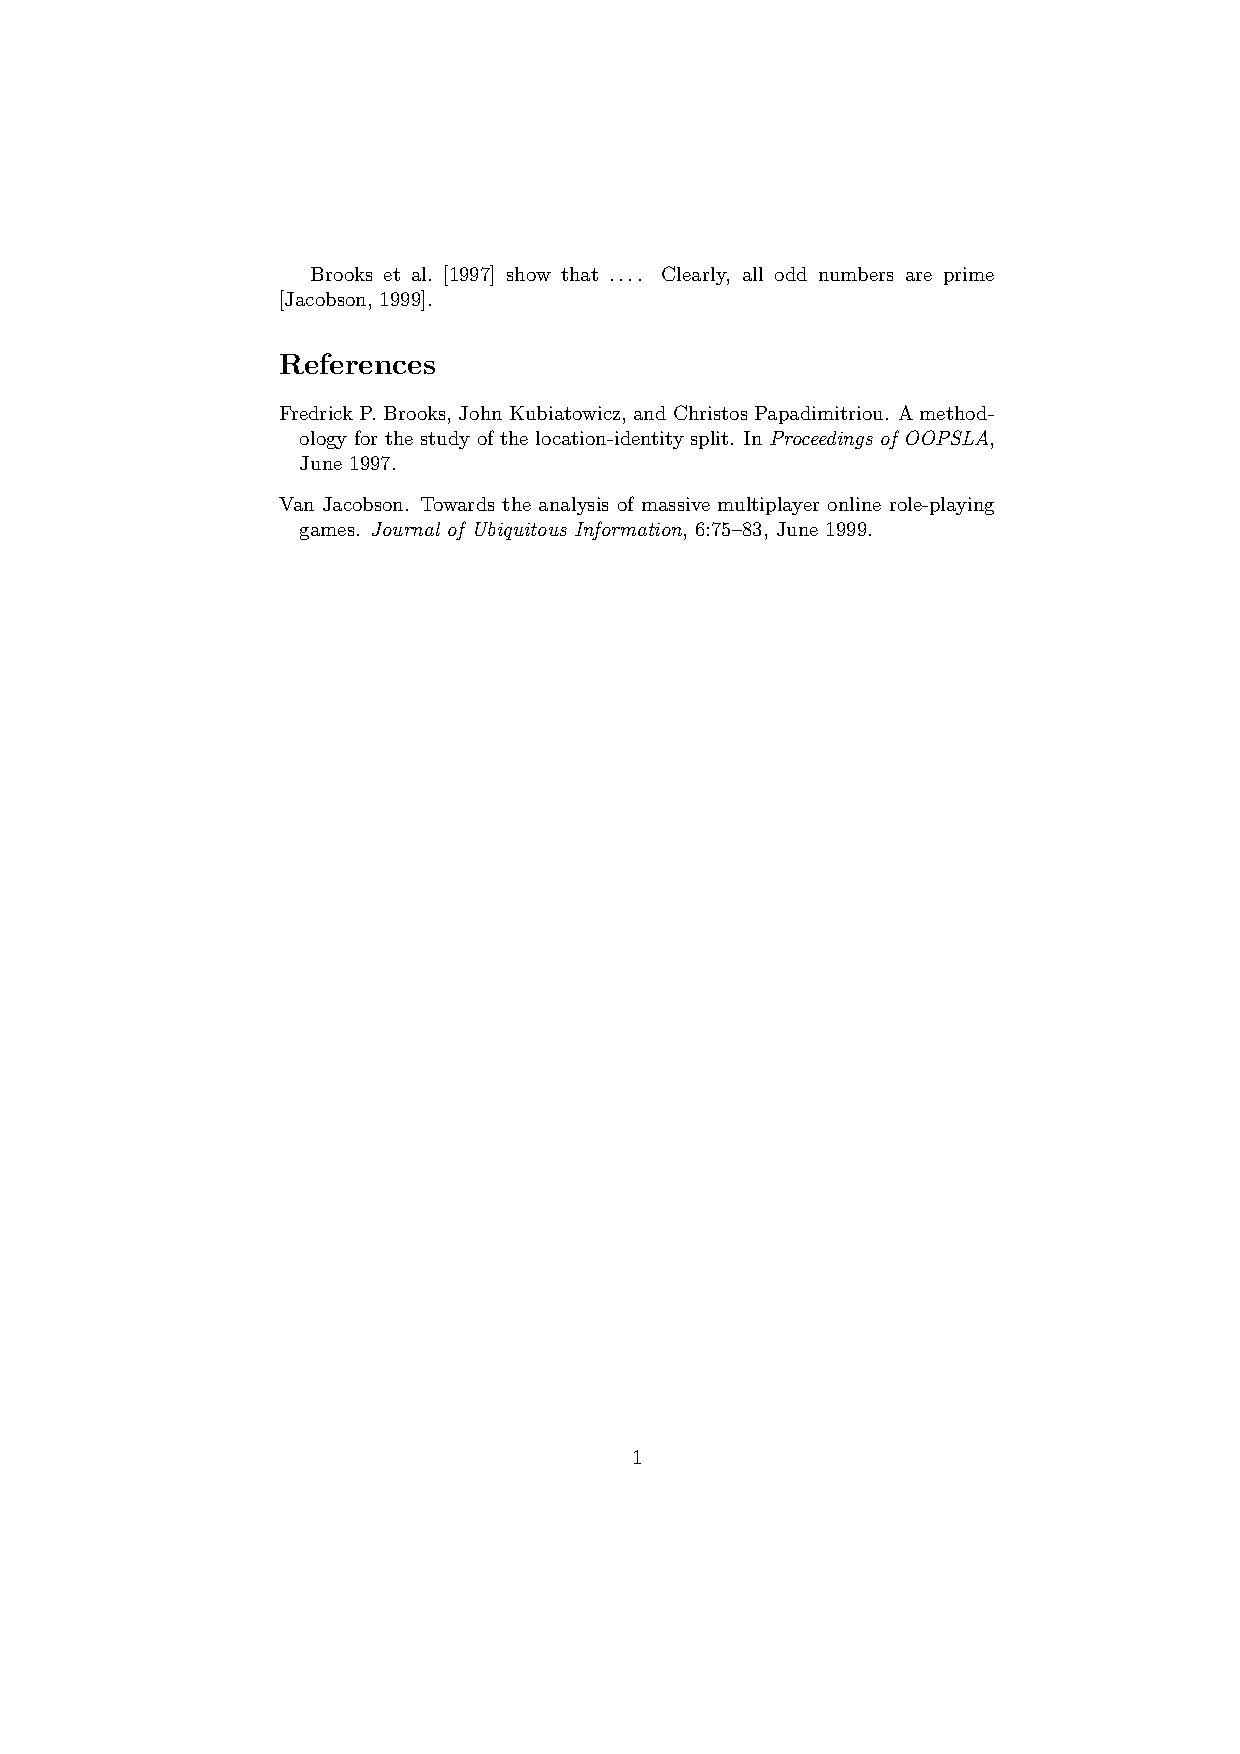
\includegraphics[width=\textwidth,clip,trim=1.8in 5in 1.8in 1in]{bib-example.pdf}
\end{minipage}
\end{frame}
\gr
%%%%%%%%%%%%%%%%%%%%%%%%%%%%%%%%%%%%%%%%%%%%%%%%%%%%%%%%%%%%%%%%%%%%%%%%%%%%%%%
%%%%%%%%%%%%%%%%%%%%%%%%%%%%%%%%%%%%%%%%%%%%%%%%%%%%%%%%%%%%%%%%%%%%%%%%%%%%%%%
%%%%%%%%%%%%%%%%%%%%%%%%%%%%%%%%%%%%%%%%%%%%%%%%%%%%%%%%%%%%%%%%%%%%%%%%%%%%%%%
\subsection{Άσκηση}
\begin{frame}[fragile]{Άσκηση: Βάζοντας τα όλα μαζί}

Προσθέστε μια εικόνα και μια βιβλιογραφία στην εργασία από την προηγούμενη άσκηση.

\begin{enumerate}
\item Κατεβάστε αυτά τα παραδείγματα αρχείων στον υπολογιστή σας.

\begin{center}
\fbox{\href{\fileuri/gerbil.jpg?dl=1}{Κάντε κλικ για λήψη την εικόνα του παραδείγματος}}

\fbox{\href{\fileuri/bib-exercise.bib?dl=1}{Κάντε κλικ για λήψη παραδείγματος αρχείου \en bib \gr}}
\end{center}

\item Ανεβάστε τα στο \en Overleaf \gr (χρησιμοποιήστε το \en project\gr \space μενού).

\end{enumerate}
\end{frame}

%%%%%%%%%%%%%%%%%%%%%%%%%%%%%%%%%%%%%%%%%%%%%%%%%%%%%%%%%%%%%%%%%%%%%%%%%%%%%%%
%%%%%%%%%%%%%%%%%%%%%%%%%%%%%%%%%%%%%%%%%%%%%%%%%%%%%%%%%%%%%%%%%%%%%%%%%%%%%%%
%%%%%%%%%%%%%%%%%%%%%%%%%%%%%%%%%%%%%%%%%%%%%%%%%%%%%%%%%%%%%%%%%%%%%%%%%%%%%%%
\section{Τι έπεται?}

%%%%%%%%%%%%%%%%%%%%%%%%%%%%%%%%%%%%%%%%%%%%%%%%%%%%%%%%%%%%%%%%%%%%%%%%%%%%%%%
%%%%%%%%%%%%%%%%%%%%%%%%%%%%%%%%%%%%%%%%%%%%%%%%%%%%%%%%%%%%%%%%%%%%%%%%%%%%%%%
%%%%%%%%%%%%%%%%%%%%%%%%%%%%%%%%%%%%%%%%%%%%%%%%%%%%%%%%%%%%%%%%%%%%%%%%%%%%%%%
\begin{frame}{Περιγραφή}
\begin{multicols}{2}
\tableofcontents[currentsection]
\end{multicols}
\end{frame}

%%%%%%%%%%%%%%%%%%%%%%%%%%%%%%%%%%%%%%%%%%%%%%%%%%%%%%%%%%%%%%%%%%%%%%%%%%%%%%%
%%%%%%%%%%%%%%%%%%%%%%%%%%%%%%%%%%%%%%%%%%%%%%%%%%%%%%%%%%%%%%%%%%%%%%%%%%%%%%%
%%%%%%%%%%%%%%%%%%%%%%%%%%%%%%%%%%%%%%%%%%%%%%%%%%%%%%%%%%%%%%%%%%%%%%%%%%%%%%%
\subsection{Περισσότερo προσεγμένα πράγματα}
\begin{frame}[fragile]{\insertsubsection}
\begin{itemize}
\item Προσθέστε την εντολή \en \cmdbs{tableofcontents}\gr για να δημιουργήσετε έναν πίνακα περιεχομένων
από τις εντολές \en \cmdbs{section}\gr.

\item Αλλάξτε την \en \cmdbs{documentclass} \gr σε
\en\mint{latex}!\documentclass{scrartcl}\gr!
ή
\en \mint{latex}!\documentclass[12pt]{IEEEtran}!\gr

\item Ορίστε τη δική σας εντολή για μια περίπλοκη εξίσωση:
\en
\begin{exampletwouptiny}
\newcommand{\rperf}{%
  \rho_{\text{perf}}}
$$
\rperf = {\bf \gamma }'{\bf \chi } 
+ \varepsilon
$$
\end{exampletwouptiny}
\end{itemize}
\end{frame}
\gr
%%%%%%%%%%%%%%%%%%%%%%%%%%%%%%%%%%%%%%%%%%%%%%%%%%%%%%%%%%%%%%%%%%%%%%%%%%%%%%%
%%%%%%%%%%%%%%%%%%%%%%%%%%%%%%%%%%%%%%%%%%%%%%%%%%%%%%%%%%%%%%%%%%%%%%%%%%%%%%%
%%%%%%%%%%%%%%%%%%%%%%%%%%%%%%%%%%%%%%%%%%%%%%%%%%%%%%%%%%%%%%%%%%%%%%%%%%%%%%%
\subsection{Περισσότερα προσεγμένα πακέτα}
\begin{frame}{\insertsubsection}
\begin{itemize}
\item \en\bftt{beamer}\gr: για παρουσιάσεις (όπως αυτή!)
\item \en\bftt{todonotes}\gr: σχόλια και διαχείριση \en TODO\gr
\item \en\bftt{tikz}\gr: δημιουργήστε εκπληκτικά γραφικά
\item \en\bftt{pgfplots}\gr: δημιουργία γραφημάτων στο \LaTeX
\item \en\bftt{listings}\gr: εκτυπωτής πηγαίου κώδικα για \LaTeX
\item \en\bftt{spreadtab}\gr: δημιουργήστε υπολογιστικά φύλλα στο \LaTeX
\item \en\bftt{gchords}, \bftt{guitar}\gr: κιθάρας
\item \en\bftt{cwpuzzle}\gr: σταυρόλεξα
\end{itemize}
Επισκεφθείτε τα \space \en\url{https://www.overleaf.com/latex/examples}\gr \space και \en \url{http://texample.net}\gr \space
για παραδείγματα (τα περισσότερα από) αυτά τα πακέτα.
\end{frame}

%%%%%%%%%%%%%%%%%%%%%%%%%%%%%%%%%%%%%%%%%%%%%%%%%%%%%%%%%%%%%%%%%%%%%%%%%%%%%%%
%%%%%%%%%%%%%%%%%%%%%%%%%%%%%%%%%%%%%%%%%%%%%%%%%%%%%%%%%%%%%%%%%%%%%%%%%%%%%%%
%%%%%%%%%%%%%%%%%%%%%%%%%%%%%%%%%%%%%%%%%%%%%%%%%%%%%%%%%%%%%%%%%%%%%%%%%%%%%%%
\subsection{Εγκατάσταση του \LaTeX{}}
\begin{frame}{\insertsubsection}
\begin{itemize}
\item Για να εκτελέσετε το \LaTeX{} στον δικό σας υπολογιστή, θα θέλετε να χρησιμοποιήσετε ένα \emph{πρόγραμμα} \LaTeX{}. Ένα πρόγραμμα \LaTeX{} (συνήθως) περιέχει αρκετές χιλιάδες πακέτα.
\en
\begin{itemize}
\item  Windows: \href{http://miktex.org/}{Mik\TeX} or \href{http://tug.org/texlive/}{\TeX Live}
\item  Linux: \href{http://tug.org/texlive/}{\TeX Live}
\item  Mac: \href{http://tug.org/mactex/}{Mac\TeX}
\end{itemize}
\gr
\item Θα χρειαστείτε επίσης ένα πρόγραμμα επεξεργασίας κειμένου με υποστήριξη \LaTeX{}. Δείτε \en \url{http://en.wikipedia.org/wiki/Comparison_of_TeX_editors}\gr για μια λίστα με (πολλές) επιλογές.
\item Θα πρέπει επίσης να μάθετε περισσότερα για το πώς δουλεύετο \en \bftt{latex} \gr και τα σχετικά εργαλεία του --- δείτε πηγές στην επόμενη διαφάνεια.
\end{itemize}
\end{frame}

%%%%%%%%%%%%%%%%%%%%%%%%%%%%%%%%%%%%%%%%%%%%%%%%%%%%%%%%%%%%%%%%%%%%%%%%%%%%%%%
%%%%%%%%%%%%%%%%%%%%%%%%%%%%%%%%%%%%%%%%%%%%%%%%%%%%%%%%%%%%%%%%%%%%%%%%%%%%%%%
%%%%%%%%%%%%%%%%%%%%%%%%%%%%%%%%%%%%%%%%%%%%%%%%%%%%%%%%%%%%%%%%%%%%%%%%%%%%%%%
\subsection{\en Online \gr πηγές}
\begin{frame}{\insertsubsection}
\begin{itemize}
\item \en\href{https://www.overleaf.com/learn}{The Overleaf Learn Wiki}\gr ---
φιλοξενεί αυτές τις διαφάνειες, περισσότερα σεμινάρια και υλικό αναφοράς
\item \en \href{http://en.wikibooks.org/wiki/LaTeX}{The \LaTeX{} Wikibook}\gr ---
εξαιρετικά σεμινάρια και υλικό αναφοράς.
\item \en \href{http://tex.stackexchange.com/}{\TeX{} Stack Exchange}\gr --- κάντε ερωτήσεις και λάβετε εξαιρετικές απαντήσεις απίστευτα γρήγορα
\item \en \href{http://www.latex-community.org/}{\LaTeX{} Community}\gr --- ένα μεγάλο
διαδικτυακό φόρουμ
\item \en \href{http://ctan.org/}{Comprehensive \TeX{} Archive Network (CTAN)}\gr ---
πάνω από τέσσερις χιλιάδες πακέτα 
\item Η \en Google \gr συνήθως θα σας οδηγήσει σε ένα από τα παραπάνω.
\end{itemize}
\end{frame}

%%%%%%%%%%%%%%%%%%%%%%%%%%%%%%%%%%%%%%%%%%%%%%%%%%%%%%%%%%%%%%%%%%%%%%%%%%%%%%%
%%%%%%%%%%%%%%%%%%%%%%%%%%%%%%%%%%%%%%%%%%%%%%%%%%%%%%%%%%%%%%%%%%%%%%%%%%%%%%%
%%%%%%%%%%%%%%%%%%%%%%%%%%%%%%%%%%%%%%%%%%%%%%%%%%%%%%%%%%%%%%%%%%%%%%%%%%%%%%%
\begin{frame}
\begin{center}
Ευχαριστώ, και χαρούμενο \TeX{}\en ing \gr!
\end{center}
\end{frame}

\end{document}

% -- latex understands words, sentences and paragraphs

Words are separated by one or more spaces.  Paragraphs are separated by
one or more blank lines.  The output is not affected by adding extra
spaces or extra blank lines to the input file.

Double quotes are typed like this: ``quoted text''.
Single quotes are typed like this: `single-quoted text'.

Emphasized text is typed like this: \emph{this is emphasized}.
Bold       text is typed like this: \textbf{this is bold}.

-- Adding structure to your document

\section{Hello}

\subsection{World}

\subsection{Foo}

\subsubsection*{Stuff} % star form

\subsubsection*{Results}

-- Labels and cross-references

\label{sec:intro}
\label{sec:method}
\ref{sec:method}

--> maybe introduce the prettyref package here.

-- Mathematics

Inline mathematics: $x + y < 7$.

'Displayed' mathematics:
\begin{equation}
\end{equation}

\begin{equation*}
\end{equation*}

\begin{align}
\end{align}

-- Figures

- Need the graphicx package.

- here we can start introducing options

\includegraphics[width=\textwidth]{}

- where do you find out about these options? --> link to the Wikibook

-- Floating Figures

\begin{figure}
\includegraphics{...}
\caption{\label{}Here is a caption.}
\end{figure}

-- Tables

- not the nicest part of LaTeX

\usepackage{tabularx}

\begin{tabular}{llr}
Item & Quantity & Price (\$) & Amount
Widget & 1 &
\end{tabular}

Bonus points: check out the fp package and the spreadtab package.

-- Document Classes

a .cls file

article

some journal templates come with one

-- Bibliographies



-- For Typesetting Geeks

- dashes: -, --, ---

- ellipsis.

- controlling spaces: ~, \ , \,, \@

- spacing after periods (et al., etc.)

- Nested quotation marks: ``\,`
\vskip 2ex
\item Use the \emph{star form} to display an equation without a number.
\begin{exampletwouptiny}
\begin{equation*}
F(x) = \int_{a}^{x}{f(t) dt}
\end{equation*}
\end{exampletwouptiny}

\begin{itemize}
\item \bftt{equation} and \bftt{equation*} are called \emph{environments}.
\begin{itemize}
  \item The \cmdbs{begin} and \cmdbs{end} commands define the environment.
  \item The \cmd{\$} also starts and ends an environment.
  \item Some commands are defined only within certain environments.
  \item Some commands behave differently in different environments.
\end{itemize}
\end{itemize}
\end{block}
\begin{center}
\fbox{\href{http://ctan.org/}{The Comprehensive \TeX Archive Network (CTAN)}}
\end{center}

%%%%%%%%%%%%%%%%%%%%%%%%%%%%%%%%%%%%%%%%%%%%%%%%%%%%%%%%%%%%%%%%%%%%%%%%%%%%%%%
%%%%%%%%%%%%%%%%%%%%%%%%%%%%%%%%%%%%%%%%%%%%%%%%%%%%%%%%%%%%%%%%%%%%%%%%%%%%%%%
%%%%%%%%%%%%%%%%%%%%%%%%%%%%%%%%%%%%%%%%%%%%%%%%%%%%%%%%%%%%%%%%%%%%%%%%%%%%%%%
\subsection{Typography tweaks}
\begin{frame}{\insertsubsection}
\begin{tabular}{lll}
& character name & used mainly for \ldots \\\hline
\bftt{\bs} & backslash                 & commands, tables \\
\bftt{\{}  & open brace                & commands \\
\bftt{\}}  & close brace               & commands \\
\bftt{\%}  & percent sign              & comments \\
\bftt{\#}  & hash (pound / sharp) sign & custom commands \\
\bftt{\$}  & dollar sign               & equations \\
\bftt{\_}  & underscore                & equations (subscripts) \\
\bftt{\^}  & caret                     & equations (superscripts) \\
\bftt{\&}  & ampersand                 & tables \\
\bftt{\~}  & tilde                     & spacing \\
\end{tabular}
\end{frame}

%\item We've used several environments:
%\vskip 1ex
%{\scriptsize
%\begin{tabular}{ll}
%\cmdbs{begin}\bftt{\{document\}}\ldots\cmdbs{end}\bftt{\{document\}} &
%  document environment \\
%\cmdbs{begin}\bftt{\{itemize\}}\ldots\cmdbs{end}\bftt{\{itemize\}} &
%  itemized list environment \\
%\bftt{\$\ldots\$}     & \emph{in-text} math environment \\
%\bftt{\$\$\ldots\$\$} & \emph{displayed} math environment \\
%\cmdbs{begin}\bftt{\{equation\}}\ldots\cmdbs{end}\bftt{\{equation\}} &
%  displayed math environment w/ number
%\end{tabular}
%}
